\documentclass[11pt,a4paper]{article}
\usepackage[margin=2.5cm]{geometry}
\usepackage{amsmath,amssymb,amsthm}
\usepackage{booktabs,array,graphicx}
\usepackage[T1]{fontenc}
\usepackage{lmodern}
\usepackage{xcolor}
\usepackage[authoryear,round]{natbib}
\usepackage{xr-hyper}
\usepackage[colorlinks=true,linkcolor=blue!50!black,citecolor=blue!50!black,urlcolor=blue!50!black]{hyperref}
\usepackage{setspace}
\onehalfspacing

% Items the author must resolve before submission appear in red.
\newcommand{\todo}[1]{{\color{red}[TODO: #1]}}

\newcommand{\E}{\mathbb{E}}
\renewcommand{\Pr}{\mathbb{P}}
\newcommand{\T}{^{\top}}
\newcommand{\WIN}{WIN\$}
\DeclareMathOperator{\VaR}{VaR}

\theoremstyle{plain}
\newtheorem{theorem}{Theorem}
\newtheorem{proposition}{Proposition}
\newtheorem{lemma}{Lemma}
\newtheorem{corollary}{Corollary}
\theoremstyle{remark}
\newtheorem{remark}{Remark}

\externaldocument[M-]{../paper/2026_GIORNO_TSALLIS_HMM6_PAPER_A_JFECONOMETRICS}
\renewcommand{\thesection}{S\arabic{section}}\renewcommand{\thetable}{S\arabic{table}}\renewcommand{\thefigure}{S\arabic{figure}}
\title{Online Supplement to\\ ``When Can Market Regimes Improve Value at Risk?\\ A Proposed Information Bound for Student-$t$ Hidden Markov Models Identification''}
\author{Joilson Giorno}
\date{\today}
\begin{document}
\maketitle
\noindent This supplement reports the material summarised in the main paper. References to Theorem~1, Lemma~1, Corollary~1, Proposition~1, equations, Figure~1 and Tables~1--3, and to Sections~1--7, are to the main paper; tables and figures numbered S1, S2, \dots\ and sections S1--S6 are in this supplement. S1 describes the known-generator study and the distribution of fitted persistence; S2 the comparison with 19 conventional models and the EGARCH repair; S3 the numerical checks of the theory, the identification-collapse study and the size and power of the test; S4 the intraday forecast comparisons; S5 the daily replication; S6 the code.

\section{Known-generator study: design and recovery of persistence}\label{sec:dgp}

\subsection{Design}
We draw 500 independent paths of length 6{,}000 from each of eight prespecified centred Student-$t$ HMM conditions (4{,}000 paths in total): a calibration anchor with clearly separated scale and tail regimes; a full HMM; scale-only switching; tail-only switching at equal conditional variance; weak tail contrast; weak persistence; an independent mixture ($\rho=0$); and a single Student-$t$ (identical emissions, so transitions are unidentified). Each path is generated with a 600-observation burn-in that is discarded (the simulator draws $6{,}000+600$ observations and keeps the last 6{,}000), and the retained path is split chronologically into 4{,}800 estimation and 1{,}200 holdout observations. The six-parameter HMM is estimated without using true parameters or hidden states; labels are aligned ex post for assessment only. Bootstrap intervals describe uncertainty of means across independent paths, not coverage for individual fits.

The same 4{,}000 datasets are fitted with 19 conventional specifications: static Student-$t$, i.i.d.\ mixture, AR, MA and ARMA means, Student-$t$ GARCH, GJR \citep{glosten1993}, EGARCH \citep{nelson1991}, six power/asymmetry APARCH variants \citep{ding1993}, and a Heston--Nandi-style recursion (not the Gaussian option-pricing model of \citealp{hestonnandi2000}). The 19 specifications are listed in Table~\ref{tab:specs}. These competitors lack transition parameters and cannot recover them; their coefficients show how a misspecified model absorbs latent dependence. All likelihoods use locally written code, so independent implementation validation is still needed.

\subsection{Recovery of persistence}
\begin{table}[ht]
\centering\small
\caption{Persistence recovery under known HMM generators ($T=6{,}000$, 500 paths each)}\label{tab:rec}
\begin{tabular}{lcccccc}
\toprule
DGP & True $\rho$ & Mean $\hat\rho$ & 95\% MC interval & State acc. & Majority acc. & $\hat\nu_0\ge99$\\
\midrule
Calibration anchor & 0.900 & 0.900 & [0.899, 0.901] & 0.904 & 0.600 & 0\\
Full HMM-6 & 0.830 & 0.828 & [0.825, 0.830] & 0.884 & 0.824 & 5\\
Scale only & 0.785 & 0.784 & [0.781, 0.787] & 0.889 & 0.837 & 0\\
Tail only & 0.825 & 0.321 & [0.272, 0.366] & 0.608 & 0.857 & 66\\
Weak tail & 0.825 & 0.105 & [0.056, 0.155] & 0.452 & 0.857 & 73\\
Weak persistence & 0.190 & 0.156 & [0.106, 0.206] & 0.541 & 0.654 & 37\\
IID mixture & 0.000 & 0.186 & [0.142, 0.233] & 0.609 & 0.820 & 81\\
Single Student-$t$ & -- & -- & [--, --] & -- & -- & 33\\
\bottomrule
\end{tabular}
\par\smallskip\footnotesize\emph{Notes.} Intervals are for the mean of $\hat\rho$ over independent paths. Accuracy uses ex-post state-label matching; the majority benchmark is an ex-post constant-state classifier. ``--'' marks quantities that are not identified. The last column counts fits with aligned $\hat\nu_0\ge99$ (upper search bound 100); aligned $\hat\nu_1\ge99$ occurs in 2, 3, 5, 4 and 5 paths of the i.i.d.-mixture, scale-only, single-$t$, tail-only and weak-tail designs respectively.
\end{table}

Scale-separated regimes allow close recovery (Table~\ref{tab:rec}). Under tail-only switching the true $\rho=0.825$ but the mean estimate is $0.321$, and weak-tail switching is worse; the majority-state benchmark (0.857) beats the fitted state accuracy (0.608). The i.i.d.\ mixture has $\rho=0$ by construction, yet the HMM estimates mean $\hat\rho=0.186$. An unrestricted two-state HMM is therefore not a reliable automatic detector of Markov dependence.

The mean conceals the shape of the error (Table~\ref{tab:rhodist} and Figure~\ref{fig:rho}). In the five designs without a scale contrast, $\hat\rho$ is spread over almost the whole interval $(-0.92,\,0.97)$ at the 5th--95th percentiles. In the i.i.d.-mixture design 33\% of fitted persistences exceed $0.5$ while 34\% are negative; in the tail-only design the 75th percentile ($0.832$) is only just above the true value $0.825$, so about three quarters of paths understate persistence, and 28\% have $\hat\rho<0$. Boundary solutions do not explain this. Fits with either $\hat\nu$ at the upper bound are 37--82 of 500 in the tail-only, weak-tail, weak-persistence and i.i.d.-mixture designs, but dropping them leaves the mean slightly higher ($0.350$, $0.123$, $0.167$ and $0.235$ against $0.321$, $0.105$, $0.156$ and $0.186$). In the same four designs the fitted persistence of the boundary fits is lower ($0.130$, $0.000$, $0.029$ and $-0.061$ on average), so they pull the mean down rather than up. The false persistence is a property of the interior fits. Theorem~\ref{M-thm:persist} explains why: in these designs the estimation sample contains less than one effective observation on persistence (Section~\ref{sec:explain}).

\begin{table}[ht]
\centering\small
\caption{Distribution of fitted persistence $\hat\rho$ across 500 paths per design}\label{tab:rhodist}
\resizebox{\textwidth}{!}{%
\begin{tabular}{lcccccccccc}
\toprule
 & True & \multicolumn{5}{c}{Percentiles of $\hat\rho$} & \multicolumn{2}{c}{Share (\%)} & \multicolumn{2}{c}{$\hat\nu\ge99$ (either)}\\
\cmidrule(lr){3-7}\cmidrule(lr){8-9}\cmidrule(lr){10-11}
DGP & $\rho$ & 5 & 25 & 50 & 75 & 95 & $>0.5$ & $<0$ & Fits & Mean $\hat\rho$ without them\\
\midrule
Calibration anchor & 0.900 & 0.883 & 0.894 & 0.900 & 0.906 & 0.914 & 100 & 0 & 0 & 0.900\\
Full HMM-6 & 0.830 & 0.782 & 0.811 & 0.828 & 0.846 & 0.869 & 100 & 0 & 5 & 0.828\\
Scale only & 0.785 & 0.726 & 0.765 & 0.784 & 0.806 & 0.834 & 100 & 0 & 3 & 0.784\\
Tail only & 0.825 & -0.793 & -0.017 & 0.320 & 0.832 & 0.974 & 42 & 28 & 66 & 0.350\\
Weak tail & 0.825 & -0.916 & -0.168 & 0.096 & 0.491 & 0.967 & 25 & 41 & 73 & 0.123\\
Weak persistence & 0.190 & -0.920 & -0.160 & 0.132 & 0.619 & 0.968 & 29 & 34 & 37 & 0.167\\
IID mixture & 0.000 & -0.922 & -0.109 & 0.120 & 0.691 & 0.958 & 33 & 34 & 82 & 0.235\\
Single Student-$t$ & -- & -0.919 & -0.214 & 0.017 & 0.430 & 0.933 & 23 & 47 & 33 & 0.064\\
\bottomrule
\end{tabular}}
\par\smallskip\footnotesize\emph{Notes.} Computed from the 4{,}000 per-path fits archived with the replication package. ``Either'' counts fits with $\hat\nu_0\ge99$ or $\hat\nu_1\ge99$ before label alignment; the last column is the mean of $\hat\rho$ over the remaining fits. Persistence is invariant to state labelling. The single-$t$ design has no identified persistence; its row is shown for completeness.
\end{table}

\begin{figure}[ht]
\centering
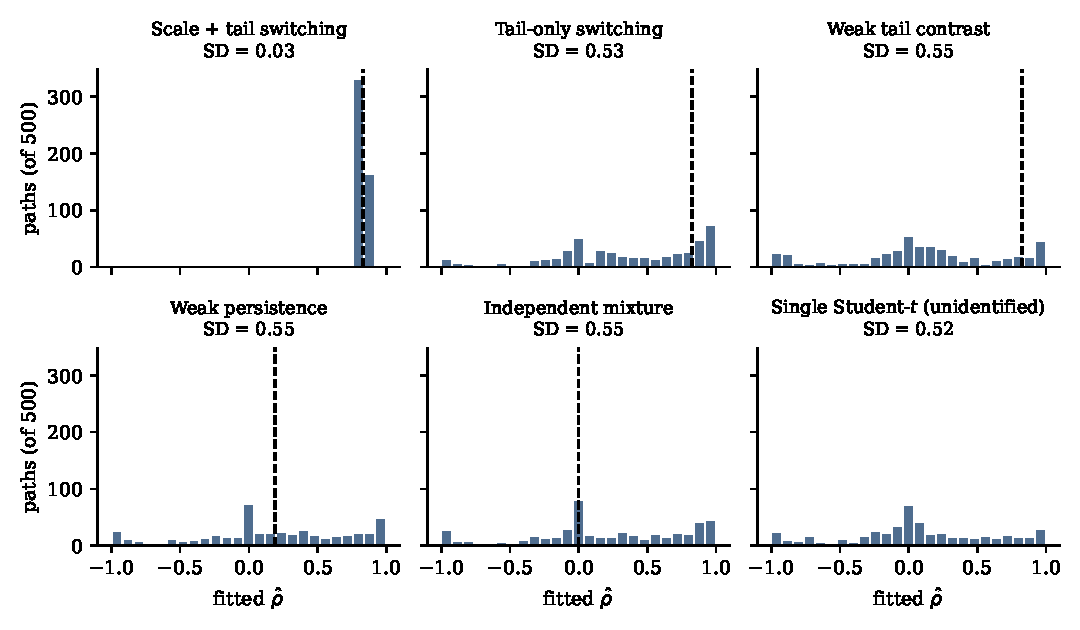
\includegraphics[width=\textwidth]{rho_hat_hist.pdf}
\caption{Distribution of fitted persistence $\hat\rho$ over 500 simulated paths per design. Dashed lines mark the true $\rho$; the single-Student-$t$ design has none because its transitions are not identified. Without a scale difference between regimes, the weak-contrast designs produce distributions close to that of the unidentified control.}\label{fig:rho}
\end{figure}

HMM optimisation reports numerical success in all 4{,}000 fits. A check against the likelihood at the true parameters flags one tail-only fit (\texttt{tail\_only\_rep0192}) whose estimation-sample likelihood is $0.252$ below the true-parameter value, an optimiser-quality warning.

\section{Conventional competitors and the EGARCH repair}\label{sec:comp}
Let $d_b=\bar\ell_{b,\rm HMM}-\bar\ell_{b,\rm comp}$ be the pathwise out-of-sample mean log-score difference. Table~\ref{tab:gain} resamples the 500 paths per DGP; these are path-level Monte Carlo intervals, not time-series tests, and the 19 comparisons per design are not adjusted for multiplicity.

\begin{table}[ht]
\centering\small
\caption{Paired out-of-sample log-score gain of the HMM over the 19 competitors}\label{tab:gain}
\resizebox{\textwidth}{!}{%
\begin{tabular}{lccccc}
\toprule
 & \multicolumn{2}{c}{Versus symmetric-power APARCH} & HMM better/tie/ & \multicolumn{2}{c}{Versus the best competitor}\\
\cmidrule(lr){2-3}\cmidrule(lr){5-6}
DGP & Mean gain & 95\% interval & worse (of 19) & Competitor & Mean gain [95\% interval]\\
\midrule
Calibration anchor & 0.028336 & [0.027814, 0.028851] & 19/0/0 & APARCH $\delta{=}1$, symmetric & 0.02818 [0.02763, 0.02870]\\
Full HMM-6 & 0.005766 & [0.005451, 0.006073] & 19/0/0 & APARCH $\delta{=}2$, symmetric & 0.00575 [0.00544, 0.00609]\\
Scale only & 0.004371 & [0.004102, 0.004651] & 19/0/0 & APARCH power, symmetric & 0.00437 [0.00410, 0.00465]\\
Tail only & 0.000018 & [$-$0.000101, 0.000131] & 4/15/0 & Static Student-$t$ & $-$0.00010 [$-$0.00022, 0.00002]\\
Weak tail & $-$0.000130 & [$-$0.000207, $-$0.000052] & 2/8/9 & Static Student-$t$ & $-$0.00025 [$-$0.00032, $-$0.00017]\\
Weak persistence & 0.000005 & [$-$0.000103, 0.000113] & 6/13/0 & Static Student-$t$ & $-$0.00007 [$-$0.00018, 0.00003]\\
IID mixture & 0.000029 & [$-$0.000083, 0.000137] & 7/12/0 & Static Student-$t$ & $-$0.00010 [$-$0.00022, 0.00001]\\
Single Student-$t$ & $-$0.000221 & [$-$0.000318, $-$0.000129] & 1/5/13 & Static Student-$t$ & $-$0.00035 [$-$0.00044, $-$0.00026]\\
\bottomrule
\end{tabular}}
\par\smallskip\footnotesize\emph{Notes.} Positive values favour the HMM; 500 paired paths per design. ``Better/tie/worse'' classifies each competitor by whether the 95\% path-bootstrap interval of the gain lies above, contains, or lies below zero. The best competitor is the one with the smallest mean gain. EGARCH enters in its repaired form ($\alpha\ge0$, all 4{,}000 paths refitted; see the EGARCH paragraph below and Table~\ref{tab:egarchgrid}); with the original specification the weak-tail and single-$t$ designs would read 3/7/9 and 2/4/13.
\end{table}

For separated scale regimes the correctly specified HMM gains clearly: it beats all 19 competitors in the calibration anchor, full-HMM and scale-only designs. In the tail-only design, where the true persistence is $0.825$, the HMM is not significantly better than a static Student-$t$ (gain $-0.00010$, interval $[-0.00022,0.00002]$) and does not beat 15 of the 19 competitors. The same holds for weak persistence and the i.i.d.\ mixture, and in the weak-tail and single-$t$ designs it is significantly worse than 9 and 13 competitors respectively, plausibly because of its additional parameters. A predictive edge over simpler models therefore does not signal the presence of latent regimes, and its absence does not rule them out. Table~\ref{tab:aparch} shows that the APARCH power estimate is near 1 for the anchor and about 1.9 for tail-only data, while the asymmetry estimate stays small relative to its Monte Carlo error. This is consistent with power adaptation \citep{ding1993} offering a competing description of some scale-switching mechanisms; it does not show that latent HMM tails always induce spurious leverage.

\begin{table}[ht]
\centering\small
\caption{Unrestricted APARCH estimates under known HMM generators (path averages)}\label{tab:aparch}
\begin{tabular}{lccc}
\toprule
DGP & Mean power $\hat\delta$ & Mean asymmetry $\hat\gamma$ & MC s.e.\ of mean $\hat\gamma$\\
\midrule
Calibration anchor & 1.001 & 0.001 & 0.002\\
Full HMM-6 & 1.721 & 0.003 & 0.003\\
Scale only & 1.712 & 0.005 & 0.003\\
Tail only & 1.923 & 0.002 & 0.031\\
Weak tail & 1.922 & 0.063 & 0.028\\
\bottomrule
\end{tabular}
\end{table}

\paragraph{EGARCH numerical failures and their repair.} Eleven EGARCH paths (four weak-tail, three weak-persistence, one i.i.d.-mixture, three single-$t$) were originally scored with a $-10^8$ sentinel because the recursion was aborted in the holdout window. We regenerated these paths from their archived seeds (the 11 estimation-sample likelihoods at the true parameters match the stored values to within $4\times10^{-10}$, the precision of the stored datasets) and refitted EGARCH with the published settings. Ten of the 11 unconstrained fits have a negative magnitude coefficient ($\hat\alpha<0$, between $-0.003$ and $-0.021$) with $\hat\beta\ge0.98$, i.e.\ they describe an almost constant variance with a wrong-signed ARCH term. Such a filter is unstable: if the fitted variance falls below the true scale, $|z_t|$ grows and a negative $\alpha$ drives the log-variance down further. In the three paths in which the refit reproduced the abort (weak-tail 437 and 455, weak-persistence 209; the original optimiser settings are not documented, so the other eight did not fail under the default settings), the recursion left the guard band $|{\log h}|\le24$ inside the holdout window (the log-variance was $-533$, $-114$ and $-50$ at the crossing step), and the remaining holdout observations received the sentinel.

The repair imposes $\alpha\ge|\gamma|$ (as a bound on $\alpha\ge0$ and an inequality constraint), the analogue of the non-negativity constraint already used for GJR. With it no sentinel remains in any of the 11 paths, the repaired holdout log scores lie between $-1.467$ and $-1.405$ (Table~\ref{tab:egarch}), and each differs from the HMM score by less than $0.002$. The constraint costs $4.5$ log-likelihood units on average in the estimation window (range $-10.7$ to $+1.0$), so the unconstrained gain came largely from the unstable region. We therefore refitted EGARCH under the sign restriction $\alpha\ge0$ on all 4{,}000 paths (same per-path seeds, five starts, 320 iterations; the EGARCH filter was run as a C routine equivalent to the archived one because the compiled library was unavailable here). No path is penalised and all 4{,}000 optimisations report success. Table~\ref{tab:egarchgrid} shows where the repair matters. In the calibration-anchor, full-HMM and scale-only designs, where the variance really moves, the fitted $\hat\alpha$ is far from zero and the HMM-minus-EGARCH gains are unchanged to five decimals ($0.0338$, $0.0065$, $0.0051$). In the five designs without a scale contrast, $\hat\alpha$ sits at the zero bound in 47--53\% of fits, i.e.\ EGARCH collapses to a constant-variance model, and the HMM's gain falls from $0.0008$--$0.0021$ to between $-0.00001$ and $0.00022$: in the weak-tail and single-$t$ designs the HMM and the repaired EGARCH are statistically tied, and elsewhere the HMM's edge is about $0.0002$ (for example, $0.00114$ to $0.00018$ in the tail-only design). Part of the HMM's earlier advantage over EGARCH in these designs was therefore produced by unstable, wrong-signed unconstrained EGARCH fits rather than by latent regimes. The 11-path analysis above imposed the stricter $\alpha\ge|\gamma|$; the full-grid refit imposes only $\alpha\ge0$, which is sufficient to remove every sentinel. Neither refit reproduces the archived unconstrained fits exactly (the original optimiser path is not recoverable), so the original EGARCH column is retained in Table~\ref{tab:egarchgrid} for comparison only. The refit scripts are supplied with the replication package.


\begin{table}[ht]
\centering\small
\caption{The 19 competing specifications (all with Student-$t$ innovations except where stated)}\label{tab:specs}
\begin{tabular}{rll}
\toprule
\# & Name & Description\\
\midrule
1 & Static-$t$ & constant mean and variance\\
2 & IIDmix-$t$ & i.i.d.\ two-component Student-$t$ mixture\\
3--4 & AR2-$t$, AR3-$t$ & AR mean, constant variance\\
5 & MA1-$t$ & MA(1) mean, constant variance\\
6--7 & ARMA11-$t$, ARMA12-$t$ & ARMA mean, constant variance\\
8 & GARCH11-normal & GARCH(1,1), Gaussian innovations\\
9 & GARCH11-$t$ & GARCH(1,1)\\
10 & GARCH12-$t$ & GARCH(1,2)\\
11 & GJR11-$t$ & GARCH with leverage term\\
12 & EGARCH11-$t$ & log-variance recursion\\
13 & APARCH11-$t$ & APARCH(1,1), power $\delta$ and asymmetry $\gamma$ free\\
14 & APARCH power, symmetric & $\gamma=0$, $\delta$ free\\
15 & APARCH $\delta{=}2$, asymmetric & $\delta=2$, $\gamma$ free\\
16 & APARCH $\delta{=}2$, symmetric & $\delta=2$, $\gamma=0$ (GARCH form)\\
17 & APARCH $\delta{=}1$, asymmetric & $\delta=1$, $\gamma$ free\\
18 & APARCH $\delta{=}1$, symmetric & $\delta=1$, $\gamma=0$\\
19 & HN11-$t$ & Heston--Nandi-style variance recursion (not option pricing)\\
\bottomrule
\end{tabular}
\par\smallskip\footnotesize\emph{Notes.} All are fitted by locally written maximum likelihood on the estimation window and scored one step ahead on the holdout; mean specifications are not combined with GARCH variance.
\end{table}
\begin{table}[ht]
\centering\small
\caption{EGARCH repair on the 11 numerically penalised paths}\label{tab:egarch}
\begin{tabular}{lccccc}
\toprule
 & \multicolumn{2}{c}{Unconstrained refit} & Abort & \multicolumn{2}{c}{Holdout log score}\\
\cmidrule(lr){2-3}\cmidrule(lr){5-6}
Path (design, replication) & $\hat\alpha$ & $\hat\beta$ & reproduced & Repaired EGARCH & HMM\\
\midrule
Weak tail, 231 & 0.0095 & 0.8790 & no & -1.4151 & -1.4139\\
Weak tail, 338 & -0.0055 & 0.9800 & no & -1.4549 & -1.4556\\
Weak tail, 437 & -0.0207 & 0.9932 & yes & -1.4048 & -1.4036\\
Weak tail, 455 & -0.0076 & 0.9983 & yes & -1.4381 & -1.4381\\
Weak persistence, 111 & -0.0151 & 0.9959 & no & -1.4353 & -1.4371\\
Weak persistence, 202 & -0.0032 & 0.9986 & no & -1.4072 & -1.4082\\
Weak persistence, 209 & -0.0074 & 0.9986 & yes & -1.4491 & -1.4489\\
IID mixture, 107 & -0.0157 & 0.9908 & no & -1.4277 & -1.4284\\
Single $t$, 337 & -0.0096 & 0.9921 & no & -1.4221 & -1.4231\\
Single $t$, 458 & -0.0086 & 0.9910 & no & -1.4517 & -1.4526\\
Single $t$, 492 & -0.0093 & 0.9935 & no & -1.4669 & -1.4674\\
\bottomrule
\end{tabular}
\par\smallskip\footnotesize\emph{Notes.} Repair: $\alpha\ge|\gamma|$. ``Abort reproduced'' marks refits that again triggered the sentinel under the default optimiser settings. Original scores were between $-1.8\times10^{6}$ and $-4.9\times10^{7}$.
\end{table}
\begin{table}[ht]
\centering\small
\caption{HMM minus EGARCH holdout log score: original versus repaired EGARCH, all 4{,}000 paths}\label{tab:egarchgrid}
\begin{tabular}{lccccc}
\toprule
 & $\hat\alpha$ at bound & Original & \multicolumn{2}{c}{Repaired ($\alpha\ge0$)} & HMM\\
\cmidrule(lr){4-5}
DGP & (\%) & mean gain & Mean gain & 95\% interval & vs EGARCH\\
\midrule
Calibration anchor & 0 & 0.03380 & 0.03380 & [0.03310, 0.03451] & better\\
Full HMM-6 & 0 & 0.00654 & 0.00654 & [0.00622, 0.00687] & better\\
Scale only & 0 & 0.00514 & 0.00514 & [0.00484, 0.00543] & better\\
Tail only & 48 & 0.00114 & 0.00018 & [0.00005, 0.00031] & better\\
Weak tail & 47 & 0.00121 & 0.00007 & [$-$0.00003, 0.00018] & tie\\
Weak persistence & 49 & 0.00113 & 0.00021 & [0.00009, 0.00034] & better\\
IID mixture & 50 & 0.00078 & 0.00022 & [0.00009, 0.00036] & better\\
Single Student-$t$ & 53 & 0.00210 & $-$0.00001 & [$-$0.00012, 0.00009] & tie\\
\bottomrule
\end{tabular}
\par\smallskip\footnotesize\emph{Notes.} Positive gains favour the HMM. ``Original'' is the archived paired summary over the valid paths (the 11 penalised paths excluded); ``repaired'' refits EGARCH on all 500 paths per design with $\alpha\in[0,1]$, five starts, 320 iterations and the original per-path seeds. The interval is a 2{,}000-draw bootstrap over paths. No repaired fit is penalised and all 4{,}000 optimisations report success. ``Better'' and ``worse'' refer to the HMM; ``tie'' means the interval contains zero.
\end{table}
\section{Checks of the theory}\label{sec:explain}

\subsection{Exact identities and small-contrast approximations}
Table~\ref{tab:kappa} evaluates the theory in the eight designs. The exact parts are confirmed. In the i.i.d.-mixture design ($T=200$, 20{,}000 paths), the finite-difference $\rho$-score at $\rho=0$ equals \eqref{M-eq:pscore} path by path (largest absolute difference $3\times10^{-7}$, correlation $1-3\times10^{-13}$), and over 100{,}000 paths its variance is $0.01115$ (bootstrap s.e.\ $0.00026$) against the exact $(T-1)\kappa^2=0.01138$. The lag-one autocorrelation of $d(Y_t)$ matches $\kappa\rho$ in all seven designs to within 1.6 Monte Carlo standard errors, and lag two matches $\kappa\rho^2$ to within 1.9. The squared returns obey the bound in (ii): their lag-one autocorrelation is $0.056$ in the calibration anchor (bound $0.354$) and indistinguishable from zero in the tail-only design (bound $0.0055$).

The effective sample size separates the designs. With $T=4{,}800$ estimation observations, $n_{\rm eff}$ is 742, 187 and 230 in the three designs with a scale contrast, where $\hat\rho$ concentrates (SD $\le0.033$). It is 0.21, 0.0002, 0.49 and 0.27 in the tail-only, weak-tail, weak-persistence and independent-mixture designs. There the sample contains less than one effective observation on persistence, and $\hat\rho$ spreads over most of the admissible range (SD 0.53--0.55). Local asymptotic standard errors are uninformative in that regime: the small-contrast information formula would give 0.30 for the tail-only design. Corollary~\ref{M-cor:detect} gives the same verdict: detecting $\rho=0.825$ with 80\% power would need $n_{\rm eff}\approx2.9$ with the most powerful test and about 9 with the lag-one score test, 14 to 43 times the tail-only value.

The small-contrast approximations are close in the weak designs but not exact at these sample sizes. At $T=2{,}000$ the simulated per-observation information for $\rho$ is $1.72\times10^{-3}$ (s.e.\ $0.10\times10^{-3}$) against $2.28\times10^{-3}$ from \eqref{M-eq:small} in the tail-only design, $2.23\times10^{-6}$ against $2.46\times10^{-6}$ for weak tails and $1.07\times10^{-4}$ against $1.19\times10^{-4}$ for weak persistence. The simulated value falls short of the leading term in every case, by about 10\% in the weak-tail and weak-persistence designs and by 25\% in the tail-only design, where $\rho$ is large and the approach to the limit is slower. In the full-HMM design, outside the small-contrast regime, it is $0.41$ against $2.19$. The predicted forecast value of persistence is below $5\times10^{-5}$ nats per observation in every weak design and matches the population gain in the tail-only design ($4.7$ against $4.3\pm0.5$, in units of $10^{-5}$). Such gains are an order of magnitude below the sampling error of a 1{,}200-observation holdout, which explains why the fitted HMM's holdout gain over the fitted i.i.d.\ mixture is indistinguishable from zero or slightly negative in these designs. In the scale-contrast designs the formula overstates the gain by a factor of two to three, as expected, but the exact population gains (0.118, 0.023 and 0.019) agree closely with the fitted holdout gains (0.119, 0.022 and 0.021).

\begin{table}[ht]
\centering\small
\caption{Regime contrast $\kappa$, effective persistence sample size and the predictions of Theorem~\ref{M-thm:persist} in the known-generator designs}\label{tab:kappa}
\resizebox{\textwidth}{!}{%
\begin{tabular}{lccrccccccc}
\toprule
 & & & & \multicolumn{2}{c}{$\mathrm{Corr}\{d(Y_t),d(Y_{t+1})\}$} & & \multicolumn{3}{c}{One-step log-score gain of persistence}\\
\cmidrule(lr){5-6}\cmidrule(lr){8-10}
DGP & $\rho$ & $\kappa$ & $T\kappa^2$ & $\kappa\rho$ (exact) & Simulated (s.e.) & SD$(\hat\rho)$ & $\tfrac12\kappa^2\rho^2/(1-\rho^2)$ & Population (s.e.) & Holdout, fitted [95\% int.]\\
\midrule
Calibration anchor & 0.900 & 0.3932 & 742 & 0.3538 & 0.3527 (0.0009) & 0.009 & $0.329$ & $0.1183$ & $0.119$ [$0.118$, $0.120$]\\
Full HMM-6 & 0.830 & 0.1975 & 187 & 0.1639 & 0.1657 (0.0013) & 0.027 & $0.0432$ & $0.02274$ & $0.0219$ [$0.0212$, $0.0227$]\\
Scale only & 0.785 & 0.2188 & 230 & 0.1717 & 0.1726 (0.0010) & 0.033 & $0.0384$ & $0.01917$ & $0.0208$ [$0.0201$, $0.0215$]\\
Tail only & 0.825 & 0.0066 & 0.212 & 0.0055 & 0.0060 (0.0008) & 0.529 & $4.7\times10^{-5}$ & $4.3\times10^{-5}$ ($5\times10^{-6}$) & $2.8\times10^{-5}$ [$-4.6\times10^{-5}$, $1.0\times10^{-4}$]\\
Weak tail & 0.825 & 0.00022 & 0.00023 & 0.00018 & $-0.0006$ (0.0005) & 0.547 & $5.1\times10^{-8}$ & $1.7\times10^{-7}$ ($2\times10^{-7}$) & $-7.1\times10^{-5}$ [$-1.4\times10^{-4}$, $-4.1\times10^{-6}$]\\
Weak persistence & 0.190 & 0.0101 & 0.494 & 0.0019 & 0.0025 (0.0007) & 0.549 & $1.9\times10^{-6}$ & $3.7\times10^{-6}$ ($1\times10^{-6}$) & $-6.5\times10^{-5}$ [$-1.4\times10^{-4}$, $1.7\times10^{-5}$]\\
IID mixture & 0.000 & 0.0076 & 0.274 & 0.0000 & 0.0000 (0.0007) & 0.554 & $0$ & $0$ & $-5.2\times10^{-5}$ [$-1.4\times10^{-4}$, $3.1\times10^{-5}$]\\
\bottomrule
\end{tabular}}
\par\smallskip\footnotesize\emph{Notes.} $\kappa=\pi_0\pi_1\int(f_0-f_1)^2/\bar f$ by numerical integration of the true emission densities; $T=4{,}800$ estimation observations. Simulated autocorrelations: 50 paths of 40{,}000 observations. ``Population'' is the mean per-observation log-likelihood difference between the true HMM and the true independent mixture over long simulated paths (no estimation); s.e.\ over paths, reported where the gain is small. ``Holdout, fitted'' is the archived out-of-sample gain of the fitted HMM over the fitted i.i.d.\ Student-$t$ mixture (\texttt{IIDmix-t}), with its path-bootstrap interval. SD$(\hat\rho)$ is from Table~\ref{tab:rhodist}. The small-contrast formula is a leading-order approximation; it is not expected to hold in the first three designs.
\end{table}

\subsection{Identification collapse across contrast and sample size}\label{sec:collapse}
Theorem~\ref{M-thm:persist} implies that contrast and sample size should matter for the precision of $\hat\rho$ mainly through $n_{\rm eff}=T\kappa^2$. We test this directly. Holding persistence at $\rho=0.825$ ($p_{00}=0.975$, $p_{11}=0.85$), we vary the contrast in two families: scale ratios $s_1/s_0\in\{1.1,1.25,1.5,2,3\}$ with $\nu_0=\nu_1=8$, and tail-only contrasts with $\nu_1=4.6$ and $\nu_0\in\{6,12,24,60\}$ at equal unit variance. For each of the 18 resulting cells we fit the six-parameter HMM, without access to the truth, to 40 paths of length $T=1{,}200$ and $4{,}800$.

Figure~\ref{M-fig:collapse} plots the standard deviation of $\hat\rho$ against $n_{\rm eff}$. The cells line up on one curve regardless of $T$ and of the type of contrast: a scale ratio of 3 with $T=1{,}200$ ($n_{\rm eff}=95$) and a ratio of 2 with $T=4{,}800$ ($n_{\rm eff}=70$) both give $0.051$. Above $n_{\rm eff}\approx5$ the dispersion follows $0.45/\sqrt{n_{\rm eff}}$; the product $\mathrm{SD}\cdot\sqrt{n_{\rm eff}}$ lies between 0.39 and 0.51 in all five such cells. Below $n_{\rm eff}\approx1$ it stays at 0.35--0.55 whatever the sample size, the uninformative band of Table~\ref{tab:rhodist}. Quadrupling $T$ does not leave that band when $\kappa$ is small: with $\nu_0=60$ the tail-only design has $n_{\rm eff}=0.09$ at $T=1{,}200$ and $0.35$ at $T=4{,}800$, and SDs of 0.35 and 0.38. The constant 0.45 is about three times the value $\{(1-\rho^2)^3/(1+\rho^2)\}^{1/2}=0.14$ implied by Proposition~\ref{M-prop:small}, consistent with that formula overstating the information at large $\rho$ (Section~\ref{sec:explain}). The collapse in $n_{\rm eff}$ away from $\rho=0$ is therefore an empirical regularity that the exact result motivates rather than implies.




\subsection{Size and power of the persistence score test}\label{sec:scoretest}
The score \eqref{M-eq:pscore} gives a simple test of independence: fit an i.i.d.\ two-component Student-$t$ mixture, compute $\hat d(Y_t)$, and compare $Z=\sqrt{T-1}\,\widehat{\mathrm{corr}}\{\hat d(Y_t),\hat d(Y_{t+1})\}$ with $N(0,1)$. Table~\ref{tab:scoretest} reports two-sided rejection rates at 5\% for $T=4{,}800$, stationary weight $\pi_0=0.7$, $\nu_0=\nu_1=8$ in the scale designs, and 100 paths per cell, together with the local power $1-\Phi(1.96-\sqrt{T-1}\,\kappa\rho)+\Phi(-1.96-\sqrt{T-1}\,\kappa\rho)$ implied by part~(iii). Size is 2--5\%, within Monte Carlo error of the nominal level, although the mixture is re-estimated on every path. Power rises with $\sqrt T\kappa\rho$ as predicted and reaches 93\% for a scale ratio of 2 and $\rho=0.4$; it falls somewhat below the local formula as $\rho$ grows, as expected for a local approximation. In the tail-only design ($\kappa=0.0097$) power stays at the size level even at $\rho=0.4$. This is the theorem's verdict, not a weakness of the test: no test can detect persistence that the data do not contain.

\begin{table}[ht]
\centering\small
\caption{Rejection rates (\%) of the contrast-autocorrelation test of $\rho=0$, $T=4{,}800$, 100 paths per cell (local-power prediction in parentheses)}\label{tab:scoretest}
\begin{tabular}{lccccc}
\toprule
Design & $\kappa$ & $\rho=0$ & $\rho=0.1$ & $\rho=0.2$ & $\rho=0.4$\\
\midrule
Scale ratio 1.5 & 0.0537 & 5 (5) & 5 (7) & 7 (12) & 19 (32)\\
Scale ratio 2 & 0.1453 & 2 (5) & 13 (17) & 45 (52) & 93 (98)\\
Tail only ($\nu$ 24 vs 4.6) & 0.0097 & 3 (5) & 3 (5) & 4 (5) & 3 (6)\\
\bottomrule
\end{tabular}
\par\smallskip\footnotesize\emph{Notes.} Two-sided test at 5\%; the mixture parameters are estimated by maximum likelihood on each path. Monte Carlo standard error about 2.2 percentage points at 5\%.
\end{table}


\paragraph{Practical implication.} Before attributing a forecast gain or a fitted $\hat\rho$ to persistent regimes, the forecaster can estimate $\hat\kappa$ from the fitted i.i.d.\ mixture, report $n_{\rm eff}=T\hat\kappa^2$, and test $\rho=0$ with the lag-one autocorrelation of $\hat d(Y_t)$, which by \eqref{M-eq:pscore} is approximately $N(0,1/T)$ under independence when the mixture family is identifiable and the nuisance parameters enter only through the marginal density. In a GARCH--HMM the states act on the standardised innovation, so (i)--(ii) apply exactly to the innovation process; with estimated volatility parameters the volatility scores are not functions of single observations, so we checked the null distribution by simulation: Section~\ref{M-sec:size} of the main text shows that both the normal critical value and a parametric bootstrap keep the size after GARCH filtering.

\section{Intraday forecasts}\label{sec:garch}

\subsection{GARCH--HMM density forecasts at 1--15 minutes}

\subsubsection{Models}
For each of two markets, WIN and a U.S.\ return series whose ticker, vendor, clock convention and adjustment are not yet independently verified, we compare three common-history variance models at M1, M5, M10 and M15:
\begin{align}
R_t&=\mu+\sqrt{h_t}Z_t,\qquad h_t=\omega+\alpha(R_{t-1}-\mu)^2+\beta h_{t-1},\\
Z_t\mid K_t=j&\sim t_{\nu_j}\Big(0,\sqrt{(\nu_j-2)/\nu_j}\Big),\qquad K_t\mid K_{t-1}\sim P.
\end{align}
G0 is GARCH with a single Student-$t$ innovation; G1 uses an independent two-component Student-$t$ mixture; G2 is the equation above, with a Markov chain on the standardised innovation tail. The variance recursion is shared and not regime-switching \citep[cf.][]{gray1996,haas2004}. With a fixed mean G2 has seven free parameters, so it is not the six-parameter HMM of Section~\ref{sec:dgp}, but Theorem~\ref{M-thm:persist} applies to its standardised innovations (Section~\ref{sec:daily}).

\subsubsection{Results}
\begin{table}[ht]
\centering\small
\caption{Mean out-of-sample log-score differences, M1--M15}\label{tab:m1m15}
\begin{tabular}{llrrrl}
\toprule
Market & Freq. & OOS $n$ & G2$-$G0 & G2$-$G1 & Best density\\
\midrule
WIN & M1 & 17{,}123 & 0.003417 & 0.002786 & G2 (GARCH--HMM)\\
U.S. & M1 & 15{,}339 & 0.001101 & 0.000995 & G2\\
WIN & M5 & 3{,}412 & 0.000171 & $-$0.000722 & G1 (i.i.d.\ mix)\\
U.S. & M5 & 3{,}002 & 0.000511 & 0.000896 & G2\\
WIN & M10 & 1{,}694 & $-$0.000760 & $-$0.000640 & G0 (GARCH--$t$)\\
U.S. & M10 & 1{,}493 & 0.002247 & 0.002224 & G2\\
WIN & M15 & 1{,}122 & $-$0.000048 & 0.000141 & G0\\
U.S. & M15 & 964 & 0.001347 & 0.000343 & G2\\
\bottomrule
\end{tabular}
\par\smallskip\footnotesize\emph{Notes.} Positive differences favour GARCH--HMM; all scores use the identical holdout within each frequency. Absolute scores are not comparable across frequencies. ``Best'' is descriptive and not adjusted for multiple testing.
\end{table}

G2 has the highest mean log score in five of eight settings (all four U.S.\ frequencies and WIN M1); G1 leads WIN M5 and G0 leads WIN M10 and M15. The count is descriptive. Holdouts shrink from about 17{,}000 to about 1{,}000 observations from M1 to M15, and the frequencies share overlapping calendar time. Observation-level holdout forecasts are available for only three cells (U.S.\ M1, U.S.\ M15 and WIN M15), where we report Diebold--Mariano-type tests \citep{diebold1995} with a HAC variance (12 lags for U.S.\ M1 and 7 for U.S.\ M15 and WIN M15) on the mean log score and on the pinball losses at the three levels, for each of the three pairwise model comparisons (36 tests). None of the nine log-score comparisons is significant (smallest two-sided $p=0.15$, G2 against G0 in U.S.\ M1), and before adjustment four of the 27 loss comparisons are significant at the 5\% level, all in U.S.\ M15; after a Holm adjustment over the 36 tests, only one survives: G2 has lower 99.5\% pinball loss than G1 in U.S.\ M15 ($z=3.45$, adjusted $p=0.020$). The Holm correction is over the available tests only and does not address the selection of cells.  We therefore do not claim that HMM tails deliver uniform improvement across markets or horizons.

For quantile forecasts at the 95\%, 99\% and 99.5\% levels (24 market--frequency--level cells, Table~\ref{tab:inv}), the lowest pinball loss is attained by G2 in 11 cells, G1 in 7 and G0 in 6. Density and quantile leadership differ: for U.S.\ M1, G2 leads on density but G0 or G1 lead at every VaR level. Unconditional coverage can be tested from the reported breach counts (Table~\ref{tab:inv}). Kupiec \citep{kupiec1995} likelihood-ratio tests of the correct exceedance rate reject at the 5\% level in 5 of 24 cells for G2, 4 for G0 and 6 for G1; after a Holm adjustment within each model, in 2, 2 and 3 cells. For G2 the rejections at 5\% are four at the 95\% level (U.S.\ M1 and M5 and WIN M15 with too few exceedances, and WIN M1 with too many) and one at 99\% (U.S.\ M1, $0.82\%$); the two that survive the adjustment are U.S.\ M1 and M5 at 95\%, both too conservative. Coverage at the 99\% and 99.5\% levels is not rejected elsewhere, but with 4--177 exceedances per cell these tests have limited power. The Christoffersen conditional-coverage tests \citep{christoffersen1998} and expected-shortfall validation require the hit sequences, which are not archived.

\subsection{Marked HMM versus static Student-$t$ for downside risk}\label{sec:var}

\subsubsection{Data and models}
The WIN\$ file has 99{,}999 adjacent-row returns, 178 date transitions and nine non-minute within-date transitions. The U.S.\ file (analysed as SPY, provenance pending) has 77{,}216 returns, 202 date transitions and 934 non-minute within-date transitions. Date changes are marked as overnight intervals with separate scale multipliers; irregular same-day intervals are not separately scaled, and an observed date change alone does not certify an exchange closure (rolls, stale prices, halts and clock changes must be checked). 

M1 is a single-regime centred Student-$t$ with common degrees of freedom, regular scale and an overnight multiplier (three parameters). M2 is a two-state centred Student-$t$ HMM with regime-specific degrees of freedom, scales and persistence plus two overnight multipliers (eight parameters). The forecast target is the next price-to-price log return, not exactly one clock minute across gaps, and the marked forecast assumes the interval class is known in advance. Both models are estimated once on the first 80\% of each sample; the HMM's predictive state probabilities use only the previous filtered state. Neither model contains a jump component; omitted jumps are left to the companion paper (Section~\ref{M-sec:disc}).

With $\VaR^{(m)}_{\alpha,t}=-Q^{(m)}_{\alpha,t}$, unconditional coverage is the share of $R_t<Q^{(m)}_{\alpha,t}$ and the pinball loss is $\rho_\alpha(R_t-Q_{\alpha,t})=(\alpha-\mathbf 1\{R_t<Q_{\alpha,t}\})(R_t-Q_{\alpha,t})$. The test samples contain 20{,}000 (WIN\$) and 15{,}444 (U.S.) returns, of which only 35 and 40 are overnight. All risk numbers are in percentage log-return units.

\subsubsection{Results}
\begin{table}[ht]
\centering\small
\caption{Out-of-sample VaR: single Student-$t$ versus marked Student-$t$ HMM}\label{tab:var}
\begin{tabular}{lcccccccc}
\toprule
 & Level & \multicolumn{2}{c}{Mean VaR (\%)} & \multicolumn{2}{c}{Violations (\%)} & Pinball & HAC\\
Market & (\%) & $t$ & HMM & $t$ & HMM & gain (\%) & $z$\\
\midrule
WIN\$ & 95 & 0.0688 & 0.0725 & 7.03 & 6.00 & 9.39 & 8.82\\
WIN\$ & 99 & 0.1441 & 0.1269 & 1.30 & 1.39 & 9.41 & 7.29\\
WIN\$ & 99.5 & 0.1930 & 0.1547 & 0.49 & 0.70 & 7.50 & 5.43\\
U.S. & 95 & 0.0520 & 0.0417 & 2.27 & 3.79 & 12.23 & 7.31\\
U.S. & 99 & 0.1020 & 0.0708 & 0.25 & 0.55 & 23.08 & 11.31\\
U.S. & 99.5 & 0.1322 & 0.0855 & 0.05 & 0.25 & 27.85 & 13.53\\
\bottomrule
\end{tabular}
\par\smallskip\footnotesize\emph{Notes.} Nominal exceedance rates are 5\%, 1\% and 0.5\%. Pinball gain $=100(\rho_t-\rho_{\rm HMM})/\rho_t$; positive values favour the HMM. HAC statistics are as reported by the estimation code and are unadjusted for multiple testing.
\end{table}

The HMM has lower average pinball loss in all six market--level comparisons, by 7.5\% to 27.9\% (Table~\ref{tab:var}). Calibration is another matter. At 99\%, WIN\$ violation rates are 1.30\% (Student-$t$) and 1.39\% (HMM) against a 1\% target, while U.S.\ rates are 0.25\% and 0.55\%. At 95\%, WIN\$ rates (7.03\%, 6.00\%) are above 5\% and U.S.\ rates (2.27\%, 3.79\%) are below it. The HMM moves the U.S.\ rates toward nominal but pushes WIN\$ rates at 99\% and 99.5\% away from it. A gain in a consistent quantile score therefore does not imply correct coverage: Kupiec tests computed from the rounded violation rates and the stated test sizes reject nominal coverage at the 1\% level in 11 of the 12 model--level pairs, including all six for the HMM; the exception is the static Student-$t$ at 99.5\% in WIN\$ ($0.49\%$ against $0.5\%$). The conclusion is insensitive to rounding: shifting each reconstructed breach count by one leaves all 11 rejections intact. At 99\% the HMM's mean VaR is lower by 0.0172 (WIN\$) and 0.0312 (U.S.) percentage-log-return units; these are model-specific buffer differences, not estimated economic losses.

\subsubsection{Tail-equality test and predictive value}
Fitting the eight-parameter HMM with separate regime degrees of freedom gives $\hat\nu_0=4.113,\hat\nu_1=4.608$ for WIN\$ and $\hat\nu_0=7.099,\hat\nu_1=4.931$ for the U.S.\ series. The signs of $\hat\nu_0-\hat\nu_1$ ($-0.495$ and $2.169$) are not comparable across markets without a common labelling rule. Equal-tail likelihood-ratio statistics are 13.42 (WIN\$) and 64.13 (U.S.), with parametric-bootstrap $p$-values of $0.0025$ ($=1/401$, the smallest attainable with 400 draws) in both cases; the null bootstrap flagged 0 and 2 problematic fits, respectively. The rejection is conditional on the fitted model and the bootstrap calibration \citep[cf.][]{hansen1992}. Profile inversion brackets the nominal 5\% boundaries for $\Delta\nu=\nu_0-\nu_1$ at $[-0.80,-0.75]$ and $[-0.25,-0.20]$ (WIN\$) and $[1.55,1.60]$ and $[2.85,2.90]$ (U.S.), but with 400 draws the Monte Carlo standard error of a $p$-value near 0.05 is about 0.011, so these brackets are provisional (Table~\ref{tab:prof}). In a single chronological holdout, separate-tail mean log scores are 1.737307 against 1.737485 for common-tail in WIN\$ (slightly worse) and 2.455295 against 2.454389 in the U.S.\ series (slightly better). In-sample evidence for different tails therefore does not guarantee predictive improvement.


\begin{table}[ht]
\centering\small
\caption{Selected bootstrap-profile grid decisions for $\Delta\nu=\nu_0-\nu_1$ ($B=400$)}\label{tab:prof}
\begin{tabular}{lcccl}
\toprule
Market & $\Delta\nu$ & Profile LR & Bootstrap $p$ & Decision at 5\%\\
\midrule
WIN\$ & $-0.80$ & 4.9835 & 0.02494 & Reject\\
WIN\$ & $-0.75$ & 3.5070 & 0.05237 & Do not reject\\
WIN\$ & $-0.25$ & 3.1820 & 0.07731 & Do not reject\\
WIN\$ & $-0.20$ & 4.6341 & 0.02743 & Reject\\
U.S. & 1.55 & 4.4510 & 0.03741 & Reject\\
U.S. & 1.60 & 3.7701 & 0.05736 & Do not reject\\
U.S. & 2.85 & 4.3127 & 0.05486 & Do not reject\\
U.S. & 2.90 & 4.9301 & 0.01995 & Reject\\
\bottomrule
\end{tabular}
\end{table}
\begin{table}[ht]
\centering\small
\caption{Full downside-tail scoring inventory of the eight intraday holdouts}\label{tab:inv}
\begin{tabular}{llcccrrr}
\toprule
Market & Freq. & Level (\%) & Best loss & G2 pinball & G2 breaches & G2 breach rate (\%) & Kupiec $p$\\
\midrule
WIN & M1 & 95 & G2 & 0.005976 & 930 & 5.431 & 0.011\\
WIN & M1 & 99 & G2 & 0.001849 & 177 & 1.034 & 0.659\\
WIN & M1 & 99.5 & G2 & 0.001097 & 96 & 0.561 & 0.270\\
U.S. & M1 & 95 & G0 & 0.002466 & 681 & 4.440 & 0.001\\
U.S. & M1 & 99 & G1 & 0.000737 & 126 & 0.821 & 0.022\\
U.S. & M1 & 99.5 & G1 & 0.000433 & 66 & 0.430 & 0.210\\
WIN & M5 & 95 & G1 & 0.012928 & 160 & 4.689 & 0.400\\
WIN & M5 & 99 & G2 & 0.003838 & 31 & 0.909 & 0.586\\
WIN & M5 & 99.5 & G2 & 0.002258 & 13 & 0.381 & 0.304\\
U.S. & M5 & 95 & G0 & 0.005699 & 111 & 3.698 & $<$0.001\\
U.S. & M5 & 99 & G0 & 0.001802 & 32 & 1.066 & 0.719\\
U.S. & M5 & 99.5 & G0 & 0.001040 & 15 & 0.500 & 0.998\\
WIN & M10 & 95 & G1 & 0.018087 & 71 & 4.191 & 0.117\\
WIN & M10 & 99 & G2 & 0.005476 & 11 & 0.649 & 0.121\\
WIN & M10 & 99.5 & G1 & 0.003278 & 8 & 0.472 & 0.870\\
U.S. & M10 & 95 & G2 & 0.008251 & 63 & 4.220 & 0.156\\
U.S. & M10 & 99 & G1 & 0.002438 & 13 & 0.871 & 0.608\\
U.S. & M10 & 99.5 & G1 & 0.001417 & 4 & 0.268 & 0.163\\
WIN & M15 & 95 & G0 & 0.022253 & 41 & 3.654 & 0.030\\
WIN & M15 & 99 & G2 & 0.007160 & 11 & 0.980 & 0.947\\
WIN & M15 & 99.5 & G2 & 0.004302 & 6 & 0.535 & 0.870\\
U.S. & M15 & 95 & G0 & 0.011093 & 38 & 3.942 & 0.118\\
U.S. & M15 & 99 & G2 & 0.003765 & 7 & 0.726 & 0.369\\
U.S. & M15 & 99.5 & G2 & 0.002429 & 4 & 0.415 & 0.700\\
\bottomrule
\end{tabular}
\par\smallskip\footnotesize\emph{Notes.} ``Best loss'' is the lowest sample-mean pinball loss in the cell (G0 GARCH--$t$, G1 GARCH--i.i.d.\ mixture, G2 GARCH--HMM), without a multiple-testing adjustment. Kupiec $p$ is the unadjusted unconditional-coverage test for G2 (Holm-adjusted values leave only U.S.\ M1 and M5 at 95\% below 0.05). All eight series share underlying market data, so cells are not independent evidence.
\end{table}
\section{Daily-frequency replication}\label{sec:daily}

\subsection{Data}
Daily WIN\$ data were not available for this revision, so the replication uses the daily open, high, low and close of the S\&P 500 index distributed with the R package \texttt{gets} \citep{pretis2018}. The data cover 3 January 1950 to 8 March 2016 and were retrieved from Yahoo Finance on 9 March 2016. We use percentage close-to-close log returns from 2 January 1990 (6{,}597 returns), and from 2000 (4{,}069 returns) as a robustness sample. Each sample uses a chronological 80/20 split.

The index open is not a traded price. In 2000--2005 it equals the previous close on 95--98\% of days, in 2006 and 2007 on 43\% and 16\%, and the artefact returns on 26, 73 and 75 days in 2011, 2012 and 2013, mostly in consecutive months. An overnight/intraday decomposition is therefore possible only from 2008 and only after dropping 199 days on which the open equals the previous close or the close. Even then the opening print is partly stale, because constituents that have not yet traded enter at their previous close. 

\subsection{GARCH--HMM on daily returns}
Table~\ref{tab:dailyA} applies the code of Section~\ref{sec:garch} to daily returns, with one change. The three G2 starting values in that code all assume persistent regimes, and on daily data all three end below the likelihood of the nested G1 model ($-7{,}085.6$ against $-7{,}084.2$ in the 1990 sample, and $-4{,}817.6$ against $-4{,}812.0$ from 2000), although G2 contains G1 as the case $p_{00}=w$, $p_{11}=1-w$. Adding a start at the fitted G1 solution raises the G2 likelihood to $-7{,}077.8$ and $-4{,}807.5$ (likelihood-ratio statistics against G1 of 12.95 and 8.86). The archived intraday summaries do not record training likelihoods, so we cannot tell whether the same local optimum affected Section~\ref{sec:garch}. 

The best daily G2 is anti-persistent: $\hat\rho=-0.37$ and $-0.29$. The heavy-tailed state ($\hat\nu_0=2.5$ and $2.3$) almost never repeats, with $\hat p_{00}$ at the lower bound of the transition parameterisation, and the other state is close to Gaussian, with $\hat\nu_1$ at its upper bound of 65. The likelihood gain over G1 therefore comes from a boundary configuration in which extreme standardised shocks are followed by near-Gaussian ones, not from persistent tail regimes, and the likelihood-ratio statistics have no standard reference distribution. Out of sample, G1 and G2 improve the mean log score over GARCH--$t$ by 0.003--0.004 per day, which is not significant (HAC $z\le1.65$), and G2 and G1 differ by at most 0.0007 (Table~\ref{tab:dailyA}). In the 2010--2016 holdout all three models have too many VaR breaches at every level, and Kupiec tests reject at 5\% in all nine cells. In the 2012--2016 holdout none is rejected (Table~\ref{tab:dailyAvar}). G2 has lower 99\% pinball loss than G1 in both samples ($z=3.31$ and $2.12$), but by only 0.4--0.6\%. Model confidence sets \citep{hansen2011} at the 90\% level (stationary bootstrap, mean block length 10, 1{,}000 draws) contain all three models for every score in both samples, except GARCH--$t$ at the 95\% level in the 1990 sample ($p=0.022$).

\begin{table}[ht]
\centering\small
\caption{Daily S\&P 500 close-to-close returns: GARCH--$t$ (G0), GARCH--i.i.d.\ mixture (G1) and GARCH--HMM (G2)}\label{tab:dailyA}
\resizebox{\textwidth}{!}{%
\begin{tabular}{lcccccccccc}
\toprule
 & & \multicolumn{4}{c}{Training log-likelihood} & \multicolumn{2}{c}{G2 estimates} & \multicolumn{3}{c}{Holdout mean log-score difference (HAC $z$)}\\
\cmidrule(lr){3-6}\cmidrule(lr){7-8}\cmidrule(lr){9-11}
Sample & Train / test & G0 & G1 & G2, original starts & G2, nested start & $\hat\rho$ & $\hat\nu_0$ / $\hat\nu_1$ & G1$-$G0 & G2$-$G0 & G2$-$G1\\
\midrule
1990--2016 & 5{,}277 / 1{,}320 & $-7094.6$ & $-7084.2$ & $-7085.6$ & $-7077.8$ & $-0.37$ & 2.51 / 65 & $0.0033$ ($1.61$) & $0.0039$ ($1.65$) & $0.0006$ ($0.66$)\\
2000--2016 & 3{,}255 / 814 & $-4823.0$ & $-4812.0$ & $-4817.6$ & $-4807.5$ & $-0.29$ & 2.32 / 65 & $0.0036$ ($1.21$) & $0.0029$ ($0.85$) & $-0.0007$ ($-0.68$)\\
\bottomrule
\end{tabular}}
\par\smallskip\footnotesize\emph{Notes.} Percentage log returns, 100$\log(C_t/C_{t-1})$; chronological 80/20 split; models, starts and evaluation code are those of the intraday study, with one added G2 start at the fitted G1 solution (``nested start''). The three original G2 starts end below the nested G1 likelihood in both samples. Under the nested start $\hat p_{00}=0.0067$ (the lower bound of the transition parameterisation) and $\hat\nu_1=65$ (the upper bound). HAC standard errors with 20 lags.
\end{table}
\begin{table}[ht]
\centering\small
\caption{Daily S\&P 500 VaR: breach rates (Kupiec $p$) and pinball-loss comparisons}\label{tab:dailyAvar}
\begin{tabular}{lcccccc}
\toprule
 & & \multicolumn{3}{c}{Breaches \% (Kupiec $p$)} & \multicolumn{2}{c}{Pinball gain of G2, HAC $z$}\\
\cmidrule(lr){3-5}\cmidrule(lr){6-7}
Sample & Level (\%) & G0 & G1 & G2 & vs G0 & vs G1\\
\midrule
1990--2016 & 95 & 6.36 (0.029) & 6.29 (0.039) & 6.36 (0.029) & $2.15$ & $0.49$\\
1990--2016 & 99 & 1.67 (0.026) & 1.82 (0.007) & 1.74 (0.014) & $0.74$ & $3.31$\\
1990--2016 & 99.5 & 0.98 (0.028) & 1.29 (0.001) & 1.14 (0.005) & $-0.59$ & $1.88$\\
2000--2016 & 95 & 5.53 (0.496) & 5.28 (0.714) & 5.28 (0.714) & $1.49$ & $0.70$\\
2000--2016 & 99 & 1.60 (0.115) & 1.60 (0.115) & 1.60 (0.115) & $1.66$ & $2.12$\\
2000--2016 & 99.5 & 0.86 (0.187) & 0.86 (0.187) & 0.86 (0.187) & $0.10$ & $1.32$\\
\bottomrule
\end{tabular}
\par\smallskip\footnotesize\emph{Notes.} Holdouts: 8 December 2010 to 8 March 2016 (1{,}320 days) and 12 December 2012 to 8 March 2016 (814 days). Positive $z$ favours G2. Unadjusted for multiple testing.
\end{table}

\subsection{What the persistence bound says about the daily fit}
Theorem~\ref{M-thm:persist} applies to the standardised GARCH innovations. From the fitted G1 mixture, $\hat\kappa=0.066$ (1990 sample) and $0.091$ (2000 sample), so the estimation samples hold $n_{\rm eff}\approx23$ and 27 effective observations on tail-regime persistence. By Corollary~\ref{M-cor:detect}, the lag-one score test could detect only $|\rho|\gtrsim0.5$ with 80\% power. The lag-one autocorrelation of the contrast $d(\hat z_t)$ in the estimation sample is $-0.067$ ($Z=\sqrt{T-1}\,\widehat{\mathrm{corr}}=-4.87$) and $-0.069$ ($Z=-3.94$). This dependence is negative, the opposite of what persistent tail regimes produce, and close to the largest magnitude a two-state HMM with these emissions allows: by part~(i), the implied persistence is $-1.02$ and $-0.76$. Because the volatility parameters are estimated, these $Z$ values are indicative rather than exact (Section~\ref{M-sec:persist}).

Two checks point to the volatility filter rather than to tail regimes. First, the squared standardised residuals are also negatively autocorrelated at lag one ($-0.017$ and $-0.055$), so the negative dependence is not specific to tail shape. Second, replacing the symmetric GARCH filter by a GJR filter \citep{glosten1993} with the same i.i.d.\ mixture raises the training log-likelihood by about 65 and 64 units, with the response to past shocks almost entirely asymmetric ($\hat\gamma=0.12$ and $0.16$, $\hat\alpha\approx0$). Leverage is a first-order feature of daily index returns that no tail-regime model on a symmetric filter can absorb. The contrast autocorrelation nevertheless stays negative under GJR ($-0.077$, $Z=-5.58$; $-0.087$, $Z=-4.95$), as does that of the squared residuals. The daily data thus provide no evidence of persistent tail regimes after volatility filtering; the dependence the HMM exploits is negative and is more plausibly a residual misfit of the variance dynamics after large shocks.

\subsection{Marked HMM versus static Student-$t$}
For the daily analogue of Section~\ref{sec:var}, a return is marked when it spans a weekend or holiday closure (21.6\% of returns), and the 3-parameter static Student-$t$ is compared with the 8-parameter marked HMM. Neither model has GARCH dynamics. The HMM finds persistent volatility regimes ($\hat p_{00}=0.9945$, $\hat p_{11}=0.9959$, scales 1.17 and 0.57, $\hat\nu$ of 4.3 and 6.8), and the marks barely matter (multipliers about 1.05). Persistence is well identified here: $\hat\kappa=0.163$ and $n_{\rm eff}=139$, as Theorem~\ref{M-thm:persist} predicts for regimes that differ in scale.

Table~\ref{tab:dailyB} reproduces the intraday pattern of Table~\ref{tab:var}. The HMM improves the holdout mean log score by 0.058 per day ($z=4.26$) and the pinball loss by 5.6\%, 18.4\% and 27.3\% at the 95\%, 99\% and 99.5\% levels ($z=1.61$, $2.89$ and $4.39$). Unlike in the intraday data, the gain coexists with acceptable coverage: HMM breach rates are 6.06\%, 1.21\% and 0.61\% (Kupiec $p=0.087$, $0.45$ and $0.60$), whereas the static model is too conservative at 99\% (0.45\%, $p=0.026$). Tail equality across regimes is rejected: the likelihood-ratio statistic is 8.06, with parametric-bootstrap $p=0.01$, the smallest attainable with 99 draws ($\chi^2_1$ reference $p=0.0045$).

The overnight/intraday version on 2008--2016 OHLC data is uninformative. Both models put the tail index at or near its lower bound (2.05--2.4), the overnight multipliers are tiny (0.03--0.16) because the index open is stale, and in a calm holdout (September 2014 to March 2016) both are far too conservative: at most one breach in 746 returns at 99\%, none at 99.5\%, and about 2.3\% at 95\%. The HMM does not improve the log score ($-0.012$, $z=-0.81$), and tail equality is not rejected (likelihood ratio 0.39, bootstrap $p=0.56$, $B=99$; three bootstrap refits had slightly negative statistics, set to zero).

\begin{table}[ht]
\centering\small
\caption{Daily S\&P 500 VaR, 2010--2016 holdout: static Student-$t$ versus marked Student-$t$ HMM (weekend/holiday marks)}\label{tab:dailyB}
\begin{tabular}{lcrcccccc}
\toprule
Level & & & \multicolumn{2}{c}{Mean VaR (\%)} & \multicolumn{2}{c}{Breaches \% (Kupiec $p$)} & Pinball & HAC\\
(\%) & Returns & $n$ & $t$ & HMM & $t$ & HMM & gain (\%) & $z$\\
\midrule
95 & All & 1{,}320 & 1.713 & 1.503 & 4.17 (0.153) & 6.06 (0.087) & 5.6 & 1.61\\
95 & Weekend/holiday & 287 & 1.752 & 1.570 & 4.88 (0.924) & 4.53 (0.710) & 8.2 & 1.45\\
99 & All & 1{,}320 & 3.343 & 2.575 & 0.45 (0.026) & 1.21 (0.453) & 18.4 & 2.89\\
99 & Weekend/holiday & 287 & 3.420 & 2.693 & 0.70 (0.585) & 1.39 (0.527) & 19.8 & 2.61\\
99.5 & All & 1{,}320 & 4.325 & 3.124 & 0.30 (0.274) & 0.61 (0.597) & 27.3 & 4.39\\
99.5 & Weekend/holiday & 287 & 4.424 & 3.268 & 0.35 (0.700) & 0.70 (0.655) & 28.4 & 2.96\\
\bottomrule
\end{tabular}
\par\smallskip\footnotesize\emph{Notes.} Close-to-close returns from 2 January 1990; estimation through 7 December 2010, holdout 8 December 2010 to 8 March 2016. A return is marked when it spans a weekend or holiday closure (21.6\% of returns). Static model: $\nu$, scale and a mark multiplier (3 parameters); HMM: $p_{00},p_{11},\nu_0,\nu_1,s_0,s_1$ and state-specific mark multipliers (8 parameters). Pinball gain $=100(\rho_t-\rho_{\rm HMM})/\rho_t$; Newey--West HAC with 20 lags; unadjusted.
\end{table}

\paragraph{Daily versus intraday.} At both frequencies a marked HMM improves quantile loss over a static Student-$t$, tail shapes differ across regimes, and GARCH--HMM density gains over simpler GARCH models are small and insignificant. The daily data add three findings. The best-fitting tail HMM on a GARCH filter is anti-persistent and lies on parameter bounds. The persistence bound shows that daily estimation samples of 3{,}255 and 5{,}277 returns contain only about 25 effective observations on tail-regime persistence. And with a volatility-regime HMM, unlike in the intraday study, the quantile-loss gain is accompanied by acceptable coverage.

\section{Code, data and reproduction}\label{sec:code}
All material is in the repository \url{https://github.com/profdrgiorno/Giorno_Tsallis_paper_A}; its README gives the commands. Each folder of \texttt{code/} has a matching folder of \texttt{results/}.
\begin{itemize}\raggedright
\item \texttt{known\_generator/}: the 4{,}000-path study (generator, competitor code, manifest, seeds, per-path fits and summaries).
\item \texttt{code/1\_theory/}: checks of Theorem~1 and Proposition~1 (Section~\ref{sec:explain}).
\item \texttt{code/2\_competitors\_egarch/}: the 19 competitors and the repaired EGARCH (Section~\ref{sec:comp}).
\item \texttt{code/3\_collapse\_and\_test/}: identification collapse (Figure~1 of the main paper) and size and power of the test (Table~\ref{tab:scoretest}).
\item \texttt{code/4\_var\_gains/}: VaR gains against $T\kappa^2$ (Table~2 of the main paper, Panels A and B).
\item \texttt{code/5\_garch\_filtered\_test/}: the regime test after GARCH filtering, with normal and bootstrap critical values.
\item \texttt{code/6\_empirical/}: daily and intraday analyses, forecast tests, and \texttt{persistence\_check.py}, which computes $\hat\kappa$, $T\hat\kappa^2$ and the test for any return series.
\end{itemize}
Market price series are not redistributed; the daily S\&P 500 data are in the R package \texttt{gets}.

% References (included directly; no BibTeX needed)
\begin{thebibliography}{}

\bibitem[Christoffersen, 1998]{christoffersen1998}
Christoffersen, P.~F. (1998).
\newblock Evaluating interval forecasts.
\newblock {\em International Economic Review}, 39(4):841--862.

\bibitem[Diebold and Mariano, 1995]{diebold1995}
Diebold, F.~X. and Mariano, R.~S. (1995).
\newblock Comparing predictive accuracy.
\newblock {\em Journal of Business \& Economic Statistics}, 13(3):253--263.

\bibitem[Ding et~al., 1993]{ding1993}
Ding, Z., Granger, C. W.~J., and Engle, R.~F. (1993).
\newblock A long memory property of stock market returns and a new model.
\newblock {\em Journal of Empirical Finance}, 1(1):83--106.

\bibitem[Glosten et~al., 1993]{glosten1993}
Glosten, L.~R., Jagannathan, R., and Runkle, D.~E. (1993).
\newblock On the relation between the expected value and the volatility of the
  nominal excess return on stocks.
\newblock {\em Journal of Finance}, 48(5):1779--1801.

\bibitem[Gray, 1996]{gray1996}
Gray, S.~F. (1996).
\newblock Modeling the conditional distribution of interest rates as a
  regime-switching process.
\newblock {\em Journal of Financial Economics}, 42(1):27--62.

\bibitem[Haas et~al., 2004]{haas2004}
Haas, M., Mittnik, S., and Paolella, M.~S. (2004).
\newblock A new approach to {M}arkov-switching {GARCH} models.
\newblock {\em Journal of Financial Econometrics}, 2(4):493--530.

\bibitem[Hansen, 1992]{hansen1992}
Hansen, B.~E. (1992).
\newblock The likelihood ratio test under nonstandard conditions: Testing the
  {M}arkov switching model of {GNP}.
\newblock {\em Journal of Applied Econometrics}, 7(S1):S61--S82.

\bibitem[Hansen et~al., 2011]{hansen2011}
Hansen, P.~R., Lunde, A., and Nason, J.~M. (2011).
\newblock The model confidence set.
\newblock {\em Econometrica}, 79(2):453--497.

\bibitem[Heston and Nandi, 2000]{hestonnandi2000}
Heston, S.~L. and Nandi, S. (2000).
\newblock A closed-form {GARCH} option valuation model.
\newblock {\em Review of Financial Studies}, 13(3):585--625.

\bibitem[Kupiec, 1995]{kupiec1995}
Kupiec, P.~H. (1995).
\newblock Techniques for verifying the accuracy of risk measurement models.
\newblock {\em Journal of Derivatives}, 3(2):73--84.

\bibitem[Nelson, 1991]{nelson1991}
Nelson, D.~B. (1991).
\newblock Conditional heteroskedasticity in asset returns: A new approach.
\newblock {\em Econometrica}, 59(2):347--370.

\bibitem[Pretis et~al., 2018]{pretis2018}
Pretis, F., Reade, J., and Sucarrat, G. (2018).
\newblock Automated general-to-specific ({GETS}) regression modeling and
  indicator saturation for outliers and structural breaks.
\newblock {\em Journal of Statistical Software}, 86(3):1--44.

\end{thebibliography}
\end{document}
